% Goals
% You can group and structure names into namespaces
% You can resolve function using argument dependent lookup
% You can create enumerations as simple types with few values
% You know how to implement your own arithmetic type and are aware of possible ambiguities

\section{Enums}
\begin{itemize}
  \itemsep -0.5em 
  \item Enums can be used for types that hold a few values.
  \item Every enum field can be converted into an int, starting with the 0. 
  \item The names of an Enum cant be given out as default. For this a lookuptable is needed.
  \item With the class keyword (Scoped Enum) the type of the enum is not visible outside the namespace. The normal unscoped Enum is visible outside the namespace.
\end{itemize}

\begin{lstlisting}[language=C++]
enum [class] <name> { 
	<enumerators>
};

enum class day_of_week {
	Mon, Tue, Wed, Thu, Fri, Sat, Sun // 0 - 6
	
	day_of_week operator++ (day_of_week & aDay) {
		int day = (aDay + 1) % (Sun + 1); // Convertion to int
		aDay = static_cast<day_of_week>(day);
		return aDay;
	}
};
\end{lstlisting}

\subsection{Arithmetic Types}
Disclaimer: You usually do not want to implement your own arithmetic types! Examples: Rings, Finite Fields.

\begin{lstlisting}
struct Ring5 {
	explicit Ring5(unsigned x = 0u)
		: val{x % 5}{} 
	unsigned value() const {
		return val; 
	}
private:
	unsigned val;
};
\end{lstlisting}


\pagebreak


\section{Namespaces}
\begin{itemize}
  \itemsep -0.5em 
  \item Namespaces are scopes for grouping and preventing name clashes.
  \item Global namespaces has the :: prefix.
  \item Nesting of namespaces is possible.
  \item Nesting of scopes allows hiding of names.
  \item Namespaces can only be defined outside of classes and functions.
  \item The same same namespace can be opened and closed multiple times.
  \item Qualified names are. used to access names in a namespace: \lstinline|demo::subdemo::foo()|
  \item A name with a leading :: is called fully qualified name: ::std::cout.
  \item \lstinline|using namespace| shouldn't be used.
\end{itemize}
%Code example 
\begin{lstlisting}[language=C++]
namespace demo {
void foo(); //1
namespace subdemo {
void foo() {/*2*/}
} // subdemo
} // demo

namespace demo {
void bar() {
  foo(); //1
  subdemo::foo(); //2
}
}

void demo::foo() { /*1*/ } // definition

int main() {
  using demo::subdemo::foo;
  foo(); //2
  demo::foo(); //1
  demo::bar();
}
	
\end{lstlisting}

\subsection{Using Declaration}
\begin{itemize}
  \itemsep -0.5em 
  \item Import a name from a namespace into the current scope
  	\SubItem{That name can be used without a namespace prefix}
  	\SubItem{Useful if the name is used very often}
  \item Alternative: using alias for types if name is long
  \item There are also using directives, which import ALL names of a namespace into the current scope.
  		\SubItem{Use them only in local scope to avoid "pollution" of your namespace.}
\end{itemize}
\begin{lstlisting}
using std::string; 
string s{"no std::"};
int main() {
	using namespace std; // local scope to avoid pollution
	cout << "Hello John";
}
\end{lstlisting}

\subsection{Anonymous Namespaces}
\begin{itemize}
  \itemsep -0.5em 
  \item Special case: omit name after namespace
  \item Implicit using directive for the chosen stream
  \item Hides modules internals
  \item Use them only in source files (*.cpp)
\end{itemize}

% Code example of Date

\subsection{Name Resolution of Namespace Members}
Types and (non-member) functions belonging to that type should be placed in a common namespace. The Advantage is \textit{Argument Dependent Lookup! ADL:} When the compiler encounter an unqualified function or operator call with an argument of a user-defined type it looks into the namespaces in which that type is defined to resolve the function\/operator. E.g. it is not necessary to write std:: in front of for\_each when std::vector::begin() is an argument of the function.

% Sample with calendar and print function that does not work.. and ADL examples

\begin{figure}[h!]
  \center
  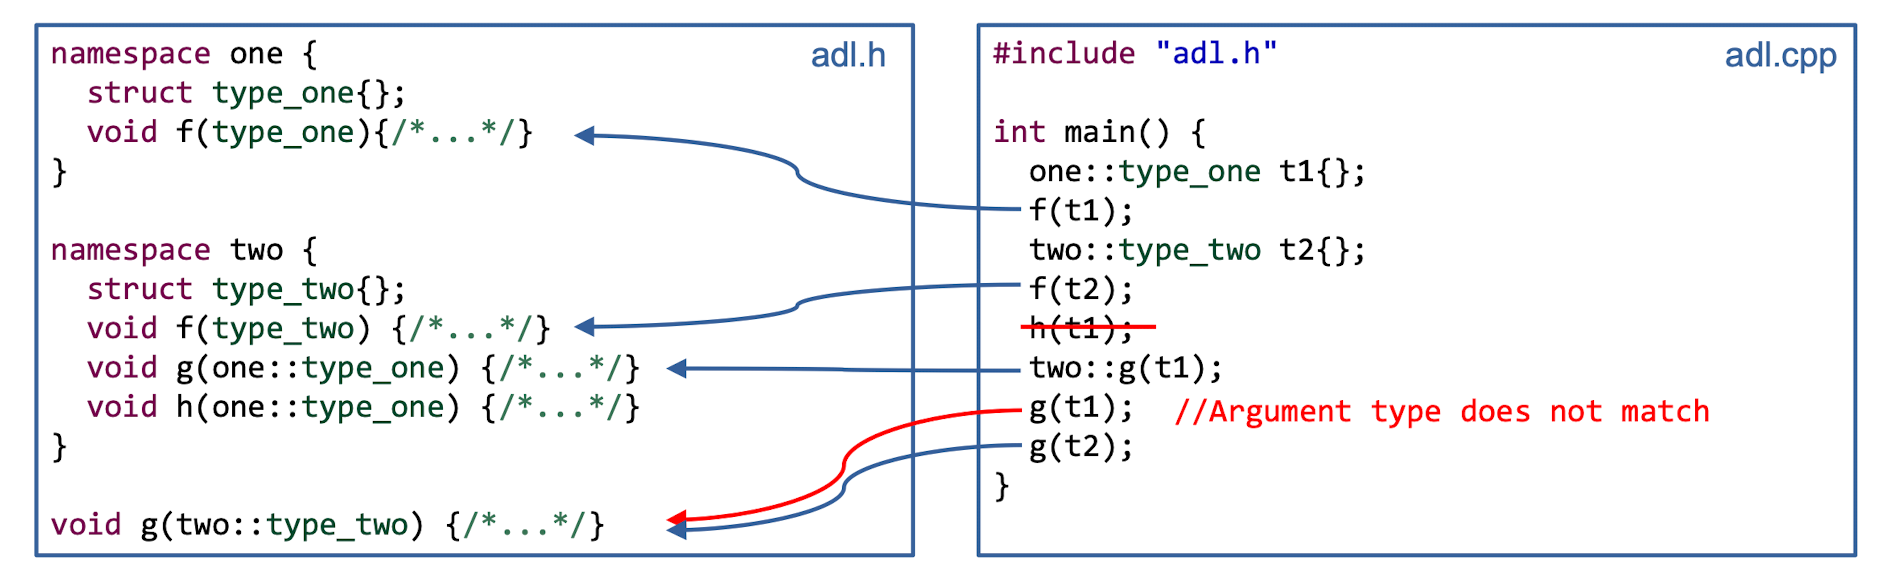
\includegraphics[width=0.75\linewidth]{adl}
  \caption{Argument Dependent Lookup Example}
\end{figure}



\subsection{Arithmetic Types}
Disclaimer: You usually do not want to implement your own arithmetic types! We will cover the basics.

\begin{itemize}
	\itemsep -0.5em
    \item Arithmetic types must be equality comparable
    \item Boost can be used to get != operator $\rightarrow$ boost::equality\_comparable
    \item It might be convenient to have the output operator
    \item Result must be in a specific range (Modulo)
\end{itemize}